\section{Quadratic Survey Interface Design}
\label{sec:interfaceDesign}
This section presents our QS interface. \change{Drawing on existing QV interfaces described in Section~\ref{sec:related_qv} and prior literature, we iterated through paper prototypes and three design pre-tests, detailed in Appendix~\ref{apdx:design}. Initially,} participants struggled to~\textit{rank} relative preferences among options and~\textit{rate} the degree of trade-offs between them. In this study, we focus on addressing the former challenge, which pertains to preference construction.

\subsection{`Organize-then-Vote': The Two-Phase Interface}
\label{sec:finalInterfaceDesign}

\subsubsection{Justifying a two-phase approach}
The main objective of the two-phase interface is to facilitate preference construction and reduce cognitive load. As shown in Figure~\ref{fig:interactiveInterface}, the interface consists of two steps: an organization phase and a voting phase. In both phases, survey respondents can drag and drop options across the presented list.

\paragraph{A two-phase approach}
Preferences are shaped through a series of decision-making processes~\cite{lichtensteinConstructionPreference2006}. Two decision-making theories~\change{inspired this} two-step interaction interface design:~\textcite{montgomeryDecisionRulesSearch1983}'s Search for a Dominance Structure Theory (Dominance Theory) and~\textcite{svensonDifferentiationConsolidationTheory1992}'s Differentiation and Consolidation Theory (Diff-Con Theory). The former suggested that decision-makers prioritize creating dominant choices to minimize cognitive effort by focusing on evidently superior options~\cite{montgomeryDecisionRulesSearch1983}. The latter described a two-phase process where decisions are formed by initially~\textit{differentiating} among alternatives and then~\textit{consolidating} these distinctions to form a stable preference~\cite{svensonDifferentiationConsolidationTheory1992}.~\change{Pre-tests showed participants puzzled by ranking all options before voting. These theories suggest decisions emerge by eliminating choices, not by fully ranking them. Therefore, the organize-then-vote design makes this natural process more explicit. Phase one} focused on differentiating and identifying dominant options, enabling survey respondents to preliminarily categorize and prioritize their choices. Phase two presented these categorized options in a comparable manner, with drag-and-drop functionality, enhancing one's ability to consolidate preferences. This structured approach aimed to construct a clear decision-making procedure that reduced cognitive load and enhanced clarity and confidence in the decisions made.

\paragraph{Phase 1: Organization Phase}
The goal of the organization phase was to support participants in identifying clearly superior options or partitioning choices into distinguishable groups. In this section, we first describe how the interaction works, then we detail the reasons for the implemented design decisions.

The organizing interface, depicted on the top half of Figure~\ref{fig:interactiveInterface}, sequentially presents each survey option. Participants select a response among three ordinal categories -- ``Lean Positive'', ``Lean Negative'', or ``Lean Neutral''. Once selected, the system moves that option to the respective category. Participants can skip the option if they do not want to indicate a preference. Options within the groups are draggable and rearrangeable to other groups should the participants wish.

To support preference formation, respondents are shown one option at a time, allowing them to either recall a prior judgment or construct a new one based on the presented choices~\cite{strackThinkingJudgingCommunicating1987}. Limiting the information presented this way also helps reduce cognitive load by preventing overload from too many options~\cite{swellerCognitiveLoadTheory2011}. This incremental process ensures that participants form opinions on individual options.

The three possible options --- Lean Positive, Lean Neutral, and Lean Negative --- aim to scaffold participants in constructing their own choice architecture~\cite{munscherReviewTaxonomyChoice2016, thalerNudgeImprovingDecisions2008a}, which strategically segments options into diverse and alternative choice presentations while avoiding biases from defaults. We believed that these three categories were sufficient for participants to segment the options. We do not limit the number of options one can place in each category to prioritize user agency, allowing participants full control over how they organize their preferences~\cite{norman2013design}. Immediate feedback displays the placement of options and allows participants to rearrange them via drag-and-drop, adhering to key interface design principles~\cite{norman2013design}. At the same time, it allows finer-grain control for individuals to surface dominating options and create differentiating groups of options.

\paragraph{Phase 2: Interactive Voting Phase}

The objective of the voting phase is to facilitate the consolidation of differentiated options through interactive elements while reinforcing the differentiation across options constructed by participants in the previous phase. This facilitation is achieved by retaining the drag-and-drop functionality for direct manipulation of position and enabling sorting within each category.

Options are displayed as they are categorized within each category from the previous step and in the following section --- Lean Positive, Lean Neutral, Lean Negative, and Skipped or Undecided --- as detailed on the bottom half of Figure~\ref{fig:interactiveInterface}. The Skipped or Undecided category contains options left in the organization queue, possibly because survey respondents have a pre-existing preference or chose not to organize their thoughts further. The original order within these categories is preserved to maintain and reinforce the differentiated options. This ordering sequence mitigated early prototype concerns where uncategorized options were left at the top of the voting interface confusing survey respondents. Respondents have the flexibility to return to the organization interface at any point during the survey to revise their choices.

In the voting interface, options are draggable, allowing participants to modify or reinforce their preference decisions as needed. Each category features a sort-by-vote function for reordering within the group, which, although it doesn’t affect the final outcome, supports information organization and consolidation. Both features aim to group similar options automatically and emphasize proximity, reducing cognitive load by following the proximity compatibility principle to enhance decision-making~\cite{wickens1990proximity}.

While multiple interaction mechanisms exist, drag-and-drop has been extensively explored in rank-based surveys. For instance,~\textcite{krosnick2018measurement} demonstrated that replacing drag-and-drop with traditional number-filling rank-based questions improved participants' satisfaction with little trade-off in their time. Similarly,~\textcite{timbrook2013comparison} found that integrating drag-and-drop into the ranking process, despite potentially reducing outcome stability, was justified by the increased satisfaction and ease of use reported by respondents. The trade-off was deemed worthwhile as QSs did not use the final position of options as part of the outcome if it significantly enhanced user satisfaction and usability~\cite{rintoulVisualAnimatedResponse}. Together, these design decisions led to our belief that a two-phase interface with direct interface manipulation could reduce the cognitive load for survey respondents to form preference decisions when completing QSs.

In addition, we made three aesthetic design decisions~\change{considering existing QV-based interfaces}. First, we removed visual elements like icons, emojis, progress bars, and vote visualizations, as prior research indicated that emojis could influence survey interpretations and reduce user satisfaction~\cite{herringGenderAgeInfluences2020, toepoelSmileysStarsHearts2019}. While effective visualizations can aid decision-making, this study does not aim to address that question. Second, all options are visible on the screen simultaneously.~\change{Prior research recommends placing all items on the voting screen to prevent overlooked votes~\cite{CenterCivicDesign}.} This echoes the proverb ``out of sight, out of mind,'' reducing where individuals might be biased toward visible options, and additional effort is required for individuals to retrieve specific information if options are hidden. Last, use a dropdown positioned to the right of each survey option for ease of access to the budget summary when determining the votes. The layout of the votes and cost was inspired by online shopping cart checkout interfaces where quantities are supplied next to the itemized costs followed by the total checkout amount.~\change{Figure~\ref{fig:btn_design} shows the two alternatives—click-based buttons (participants disliked multiple clicks) and a wheel-based design (unfamiliar to some)—and settled on the dropdown.}


\begin{figure}[ht!]
    \centering
    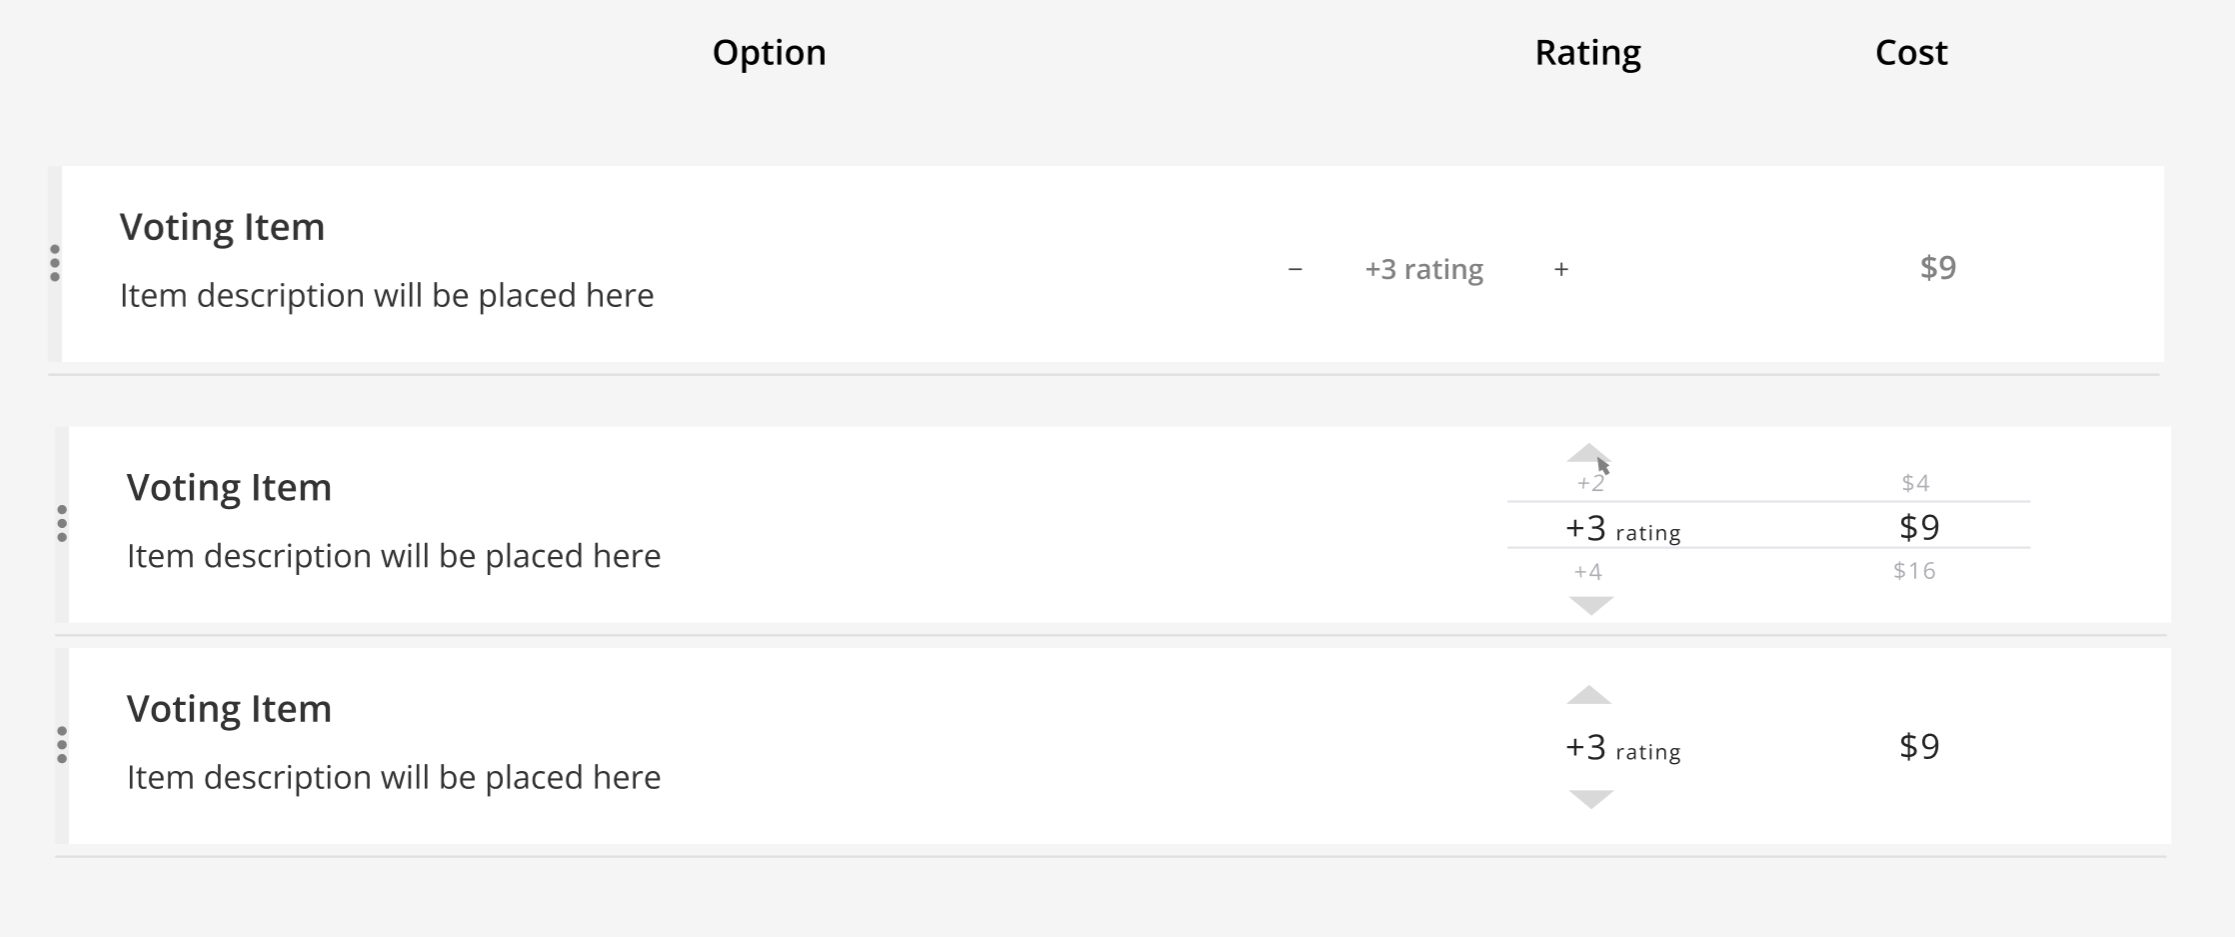
\includegraphics[width=0.8\textwidth]{content/image/prototypes/btn_design.png}
    \caption{Alternative vote control. The click-based design (upper) mirrors traditional vote control used in other QV interfaces, where each click controls one vote. The wheel-based design (the latter two) allows control through both clicks and mouse wheel rotation.}
    \Description{Three voting control interfaces are displayed. Each row represents a different interface. The first row shows a traditional click-based voting interface with options to decrease, increase, or maintain a rating of +3. The second and third rows show a wheel-based voting interface with mouse wheel functionality. In these, the middle row indicates a current rating of +3, with +2 and +4 ratings also visible. The cost for each option is listed on the right, ranging from 4 to 16. The last row mirrors the previous one with a rating of +3 and a cost of 9.}

    \label{fig:btn_design}
\end{figure}

\begin{figure}[ht]
    \centering
    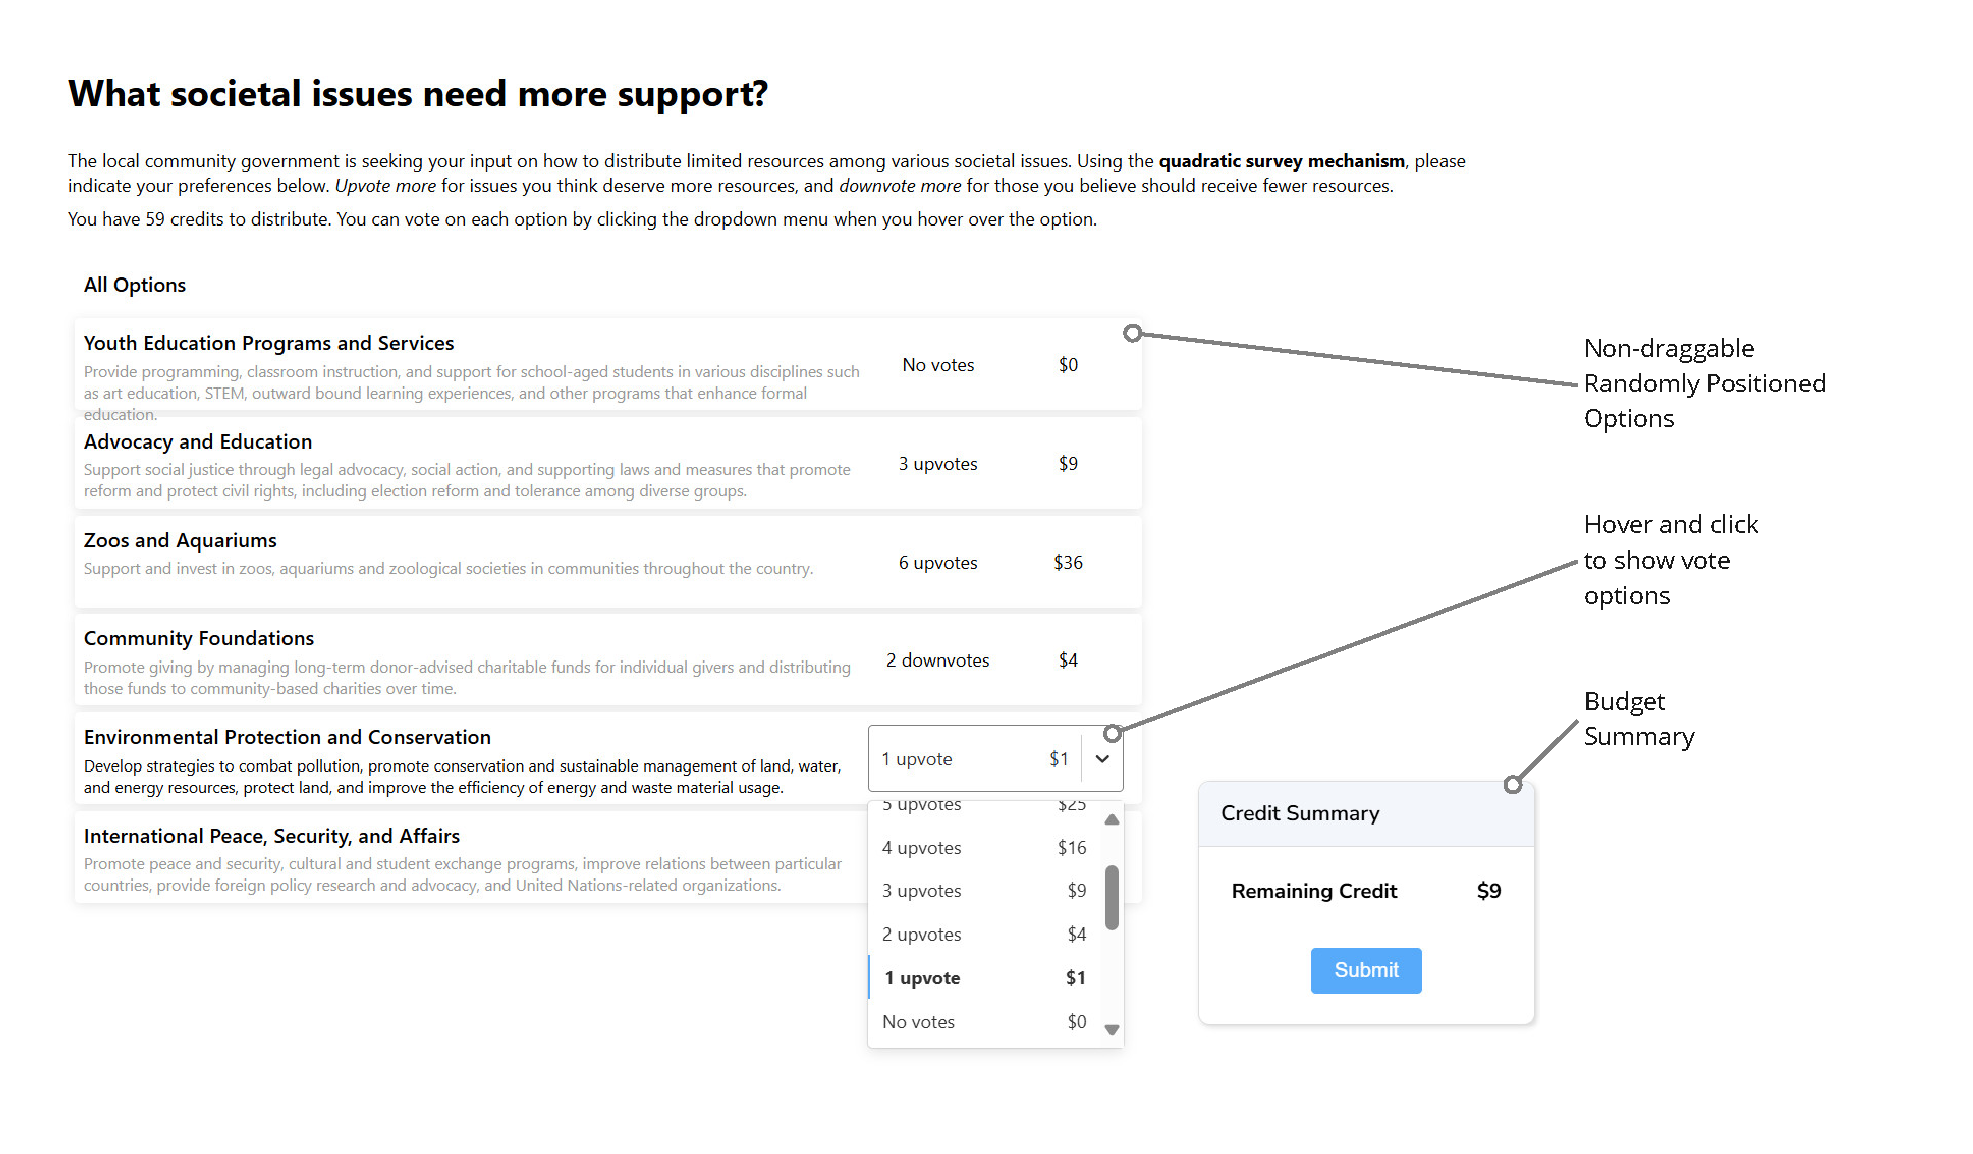
\includegraphics[width=\textwidth]{content/image/detailed_text.pdf}
    \caption{The text-based interface: This interface is based on the two-phase version but does not include the organization phase and lacks the drag-and-drop functionality. Options are randomly positioned.}
    \Description{An image of a voting interface asking users to select societal issues needing support. The title reads, "What societal issues need more support?" with a brief explanatory paragraph underneath. Below, a list of six options is displayed, including "Youth Education Programs and Services," "Advocacy and Education," "Zoos and Aquariums," "Community Foundations," "Environmental Protection and Conservation," and "International Peace, Security, and Affairs." Each option has a description, a current vote count, and a dollar amount. The right side of the image shows an expanded dropdown menu for one of the options with selectable voting choices, such as "1 upvote" and "2 upvotes." A separate box labeled "Credit Summary" shows the remaining credit of 9 and a "Submit" button below it.}
    \label{fig:textInterface}
\end{figure}

\subsection{Baseline Interface: Single-Phase Text Interface} ~\change{We created a single-phase text interface (referred to text interface for short, Figure~\ref{fig:textInterface}) as a control, enabling us to see how organizational features affect cognitive load and behavior. Like existing interfaces, it uses static lists, a summary box, and a vote control. To ensure a fair comparison, we applied the same design principles: no extraneous visuals, all options on one screen, and dropdown-based voting. The prompt appears at the top, followed by a randomly ordered list to prevent ordering bias~\cite{ferberOrderBiasMail1952, couperWebSurveyDesign2001}. Costs and the credits summary appear on the right.}

Both experimental interfaces were developed with a ReactJS frontend and a NextJS backend powered by MongoDB. We open-source both interfaces.\footnote{link-to-github}


% In our first prototyped tool, we aim to help survey respondents rank options to establish relative preferences before voting. As shown in Figure~\ref{fig:qv_rank}, our prototype allows respondents to move options before finalizing their votes. During our pretest, we found that respondents rarely moved the options and some questioned the need for a full ranking since it did not affect the QS submission. Many did not realize the options were draggable until we pointed it out. The main insight from this prototype is that creating a full rank is~\textit{not} essential for establishing~\textit{relative} preferences, leading us to consider selecting a subset of options instead of requiring a full rank among all options.

% First, we surveyed the current implementation of QV interfaces to understand the development of such tools. We presented a selection in Figure~\ref{fig:qv_interface_external}. All five interfaces retained and presented the following components:
% \begin{itemize}
%     \item Option list: A list of options contesting for votes.
%     \item Vote Controls: Two buttons to increase and decrease votes associated with each option.
%     \item Individual vote tally: A representation of votes associated with an option.
%     \item Summary: A summary that automatically calculated the cost across options and the remaining budget.
% \end{itemize}
% Now we present the final interactive interface and describe how it operates. In this subsection, we provide supporting evidence from prior literature that we previously omitted. These pieces of literature were omitted for clarity and focus in the previous subsection but will be reintroduced here. 
% We constructed a text-based interface that included all five components but removed the use of emojis (i.e., thumbs up and thumbs down present in Figure~\ref{fig:wedesignInterface}), progress bars, and other visualizations in the summary section (i.e., progress bars in Figure~\ref{fig:wedesignInterface} and~\ref{fig:chengInterface} or blocks presented in Figure~\ref{fig:rxcvotingInterface}), and the visual cues for individual vote counts (i.e., the colored counts and icons present in Figure~\ref{fig:gov4gitInterface} and~\ref{fig:chengInterface}).

% During this process, we noticed several issues. First, many survey respondents placed most options into the 'option you care about' category, defeating the design's purpose. Second, there were no indicators distinguishing between the selected and remaining options. Respondents did not notice their selections were kept at the top in the voting stage and were unsure why Step 1 was necessary if all options were shown again. This informed two takeaways: selecting options to vote on is too coarse to construct relative preferences, and there needs to be a clearer distinction and connection between the two phases.

% Feedback indicated that survey respondents are comfortable with this two-phase organize-then-vote design. Several user experience issues emerged, but they were addressable without significantly modifying this interaction structure. These issues include: First, dragging and dropping all options into different categories is cumbersome and can mislead respondents into thinking this is a ranking process, which is not the goal. Second, the position of unorganized options at the top of the voting list is counterintuitive. Third, the voting controls are disconnected from the option summaries, dividing attention between the left and right sides of the screen.

% These design decisions led to the interface shown in Figure~\ref{fig:textInterface}. 


% \subsubsection{Paper prototype: visualizing trade-offs}
% The original paper prototype aimed to help visualize survey respondents' tradeoffs among options. 
% The original paper prototype aimed to utilize visual representations to highlight the constrained availability of credit and to explain the costs and trade-offs associated with selecting each available option.
% Early on, we did not know which components made QS more difficult than other survey techniques. We began by surveying existing interfaces (Figure~\ref{fig:qv_interface_external} other than Figure~\ref{fig:gov4gitInterface} which did not exist near the writing of this paper). All four interfaces consist of these common components:
% As we were unsure what made QS more complex than other survey techniques, our investigation began with the existing interface (Figure~\ref{fig:qv_interface_external}, except Figure~\ref{fig:gov4gitInterface} which did not exist at that time. All four interfaces consist of these common components:
% \begin{itemize}
%     \item Option list: A list of options contesting for votes.
%     \item Vote Controls: Buttons to increase and decrease votes associated with each option.
%     \item Individual vote tally: A representation of votes associated with an option.
%     % \item Summary: A summary that automatically calculates the cost across options and the remaining budget.
%     \item Summary: An auto-generated summary of costs and remaining budget.
% \end{itemize}

% To brainstorm ways to help survey respondents manage trade-offs across options, we decomposed these options and explored several innovative layouts. Initially, we thought trade-offs were the core cause of cognitive load. In this paper, we show two versions of the paper prototypes in Figure~\ref{fig:qv_paper}. In both figures, costs are represented by blocks, similar to Figure~\ref{fig:rxcvotingInterface}. We imagine the survey respondents to drag and position options in the space provided unstructurally (Figure~\ref{fig:horizontal_paper}) or structurally (Fig~\ref{fig:vertical_paper}). Similar to the seminal debate on direct manipulation vs. interface agents~\cite{shneidermanDirectManipulationVs1997}, the research team was unsure how much control survey respondents should have over the positioning of the options to aid the decision-making process that considers trade-offs. Different from prior interfaces, we used placements of the interface to denote positive or negative number of votes. After several pretests, we learned that the main process participants aim to do throughout the survey is establishing~\textit{relative} preferences across the options, rather than thinking so much about trade-offs. 
% To further explore the features that contribute most to the complexity of QS, we developed two prototypes shown in Figure~\ref{fig:qv_paper}. Similar to Figure~\ref{fig:rxcvotingInterface}, these prototypes use blocks to represent costs, arranged either unstructurally (Figure~\ref{fig:horizontal_paper}) or structurally (Fig~\ref{fig:vertical_paper}), facilitating the visualization of the trade-offs. Unlike previous interfaces, we utilized the placement of the interface to denote positive or negative vote counts. Several protests indicated that participants primarily focus on establishing relative preferences among options rather than trade-offs. Therefore, in this study, we focused on enhancing designs that facilitate the establishment of relative preferences.
% the two main features of QS we identified are the relative preference through a combined presentation of rankings and ratings, and the option selection trade-offs due to total credit limits. 
% The initial prototyping involves collecting the interface designs for existing quadratic mechanism-based software. Iterative pretests informed each subsequent design. We present these iterations, which aim to enhance user experience in the preference construction process in the following sections.

% In the previous subsection, we highlighted critical prototype iterations that informed the final two-phase interactive process that defines the user journey. 
% We now present the final two-phase interface, its operations, and the supporting literature for comprehensive understanding.
% Then, We also discuss the aesthetic design choices that emerged throughout the iterations.
